\documentclass[]{article}
\usepackage{lmodern}
\usepackage{amssymb,amsmath}
\usepackage{ifxetex,ifluatex}
\usepackage{fixltx2e} % provides \textsubscript
\ifnum 0\ifxetex 1\fi\ifluatex 1\fi=0 % if pdftex
  \usepackage[T1]{fontenc}
  \usepackage[utf8]{inputenc}
\else % if luatex or xelatex
  \ifxetex
    \usepackage{mathspec}
  \else
    \usepackage{fontspec}
  \fi
  \defaultfontfeatures{Ligatures=TeX,Scale=MatchLowercase}
\fi
% use upquote if available, for straight quotes in verbatim environments
\IfFileExists{upquote.sty}{\usepackage{upquote}}{}
% use microtype if available
\IfFileExists{microtype.sty}{%
\usepackage{microtype}
\UseMicrotypeSet[protrusion]{basicmath} % disable protrusion for tt fonts
}{}
\usepackage[margin=1in]{geometry}
\usepackage{hyperref}
\hypersetup{unicode=true,
            pdftitle={Lab 3 Block 1: Kernel Meethods and Neural Networks},
            pdfauthor={Maximilian Pfundstein},
            pdfborder={0 0 0},
            breaklinks=true}
\urlstyle{same}  % don't use monospace font for urls
\usepackage{color}
\usepackage{fancyvrb}
\newcommand{\VerbBar}{|}
\newcommand{\VERB}{\Verb[commandchars=\\\{\}]}
\DefineVerbatimEnvironment{Highlighting}{Verbatim}{commandchars=\\\{\}}
% Add ',fontsize=\small' for more characters per line
\usepackage{framed}
\definecolor{shadecolor}{RGB}{248,248,248}
\newenvironment{Shaded}{\begin{snugshade}}{\end{snugshade}}
\newcommand{\KeywordTok}[1]{\textcolor[rgb]{0.13,0.29,0.53}{\textbf{#1}}}
\newcommand{\DataTypeTok}[1]{\textcolor[rgb]{0.13,0.29,0.53}{#1}}
\newcommand{\DecValTok}[1]{\textcolor[rgb]{0.00,0.00,0.81}{#1}}
\newcommand{\BaseNTok}[1]{\textcolor[rgb]{0.00,0.00,0.81}{#1}}
\newcommand{\FloatTok}[1]{\textcolor[rgb]{0.00,0.00,0.81}{#1}}
\newcommand{\ConstantTok}[1]{\textcolor[rgb]{0.00,0.00,0.00}{#1}}
\newcommand{\CharTok}[1]{\textcolor[rgb]{0.31,0.60,0.02}{#1}}
\newcommand{\SpecialCharTok}[1]{\textcolor[rgb]{0.00,0.00,0.00}{#1}}
\newcommand{\StringTok}[1]{\textcolor[rgb]{0.31,0.60,0.02}{#1}}
\newcommand{\VerbatimStringTok}[1]{\textcolor[rgb]{0.31,0.60,0.02}{#1}}
\newcommand{\SpecialStringTok}[1]{\textcolor[rgb]{0.31,0.60,0.02}{#1}}
\newcommand{\ImportTok}[1]{#1}
\newcommand{\CommentTok}[1]{\textcolor[rgb]{0.56,0.35,0.01}{\textit{#1}}}
\newcommand{\DocumentationTok}[1]{\textcolor[rgb]{0.56,0.35,0.01}{\textbf{\textit{#1}}}}
\newcommand{\AnnotationTok}[1]{\textcolor[rgb]{0.56,0.35,0.01}{\textbf{\textit{#1}}}}
\newcommand{\CommentVarTok}[1]{\textcolor[rgb]{0.56,0.35,0.01}{\textbf{\textit{#1}}}}
\newcommand{\OtherTok}[1]{\textcolor[rgb]{0.56,0.35,0.01}{#1}}
\newcommand{\FunctionTok}[1]{\textcolor[rgb]{0.00,0.00,0.00}{#1}}
\newcommand{\VariableTok}[1]{\textcolor[rgb]{0.00,0.00,0.00}{#1}}
\newcommand{\ControlFlowTok}[1]{\textcolor[rgb]{0.13,0.29,0.53}{\textbf{#1}}}
\newcommand{\OperatorTok}[1]{\textcolor[rgb]{0.81,0.36,0.00}{\textbf{#1}}}
\newcommand{\BuiltInTok}[1]{#1}
\newcommand{\ExtensionTok}[1]{#1}
\newcommand{\PreprocessorTok}[1]{\textcolor[rgb]{0.56,0.35,0.01}{\textit{#1}}}
\newcommand{\AttributeTok}[1]{\textcolor[rgb]{0.77,0.63,0.00}{#1}}
\newcommand{\RegionMarkerTok}[1]{#1}
\newcommand{\InformationTok}[1]{\textcolor[rgb]{0.56,0.35,0.01}{\textbf{\textit{#1}}}}
\newcommand{\WarningTok}[1]{\textcolor[rgb]{0.56,0.35,0.01}{\textbf{\textit{#1}}}}
\newcommand{\AlertTok}[1]{\textcolor[rgb]{0.94,0.16,0.16}{#1}}
\newcommand{\ErrorTok}[1]{\textcolor[rgb]{0.64,0.00,0.00}{\textbf{#1}}}
\newcommand{\NormalTok}[1]{#1}
\usepackage{graphicx,grffile}
\makeatletter
\def\maxwidth{\ifdim\Gin@nat@width>\linewidth\linewidth\else\Gin@nat@width\fi}
\def\maxheight{\ifdim\Gin@nat@height>\textheight\textheight\else\Gin@nat@height\fi}
\makeatother
% Scale images if necessary, so that they will not overflow the page
% margins by default, and it is still possible to overwrite the defaults
% using explicit options in \includegraphics[width, height, ...]{}
\setkeys{Gin}{width=\maxwidth,height=\maxheight,keepaspectratio}
\IfFileExists{parskip.sty}{%
\usepackage{parskip}
}{% else
\setlength{\parindent}{0pt}
\setlength{\parskip}{6pt plus 2pt minus 1pt}
}
\setlength{\emergencystretch}{3em}  % prevent overfull lines
\providecommand{\tightlist}{%
  \setlength{\itemsep}{0pt}\setlength{\parskip}{0pt}}
\setcounter{secnumdepth}{5}
% Redefines (sub)paragraphs to behave more like sections
\ifx\paragraph\undefined\else
\let\oldparagraph\paragraph
\renewcommand{\paragraph}[1]{\oldparagraph{#1}\mbox{}}
\fi
\ifx\subparagraph\undefined\else
\let\oldsubparagraph\subparagraph
\renewcommand{\subparagraph}[1]{\oldsubparagraph{#1}\mbox{}}
\fi

%%% Use protect on footnotes to avoid problems with footnotes in titles
\let\rmarkdownfootnote\footnote%
\def\footnote{\protect\rmarkdownfootnote}

%%% Change title format to be more compact
\usepackage{titling}

% Create subtitle command for use in maketitle
\newcommand{\subtitle}[1]{
  \posttitle{
    \begin{center}\large#1\end{center}
    }
}

\setlength{\droptitle}{-2em}

  \title{Lab 3 Block 1: Kernel Meethods and Neural Networks}
    \pretitle{\vspace{\droptitle}\centering\huge}
  \posttitle{\par}
    \author{Maximilian Pfundstein}
    \preauthor{\centering\large\emph}
  \postauthor{\par}
      \predate{\centering\large\emph}
  \postdate{\par}
    \date{2018-12-14}


\begin{document}
\maketitle

{
\setcounter{tocdepth}{3}
\tableofcontents
}
\section{Kernel Methods}\label{kernel-methods}

\textbf{Task:}

\begin{itemize}
\tightlist
\item
  Implement a kernel method to predict the hourly temperatures for a
  date and place in Sweden.
\item
  You are asked to provide a temperature forecast for a date and place
  in Sweden. The forecast should consist of the predicted te mperatures
  from 4 am to 24 pm in an interval of 2 hours.
\item
  Use a kernel that is the sum of three Gaussian kernels.
\item
  The first to account for the distance from a station to the point of
  interest.
\item
  The second to account for the distance between the day a temperature
  measurement was made and the day of interest.
\item
  The third to account for the distance between the hour of the day a
  temperature measurement was made and the hour of interest.
\item
  Choose an appropriate smoothing coefficient or width for each of the
  three kernels above.
\item
  Show that your choice for the kernels' width is sensible, i.e.~that it
  gives more weight to closer points. Discuss why your of definition of
  closeness is reasonable.
\item
  Instead of combining the three kernels into one by summing them up,
  multiply them. Compare the results obtained in both cases and
  elaborate on why they may differ.
\end{itemize}

\emph{Note that the file temps50k.csv may contain temperature
measurements that are posterior to the day and hour of your forecast.
You must filter such measurements out, i.e.~they cannot be used to
compute the forecast. Feel free to use the template below to solve the
assignment.}

\subsection{Kernels}\label{kernels}

This exercise uses three kernels which are combined to predict the
temperatures on a given location and day. We will have a look at those
kernels, how they're implemented and how the smooth parameters have been
selected. Before that we will have a look at one helper function which
is used by the kernels.

\subsubsection{Helper Function}\label{helper-function}

The helper function \texttt{min\_distance(a,\ b,\ ringSize)} calculates
the minimal distance between two elements on a discrete Quotient Ring.
Let's say we have the two times \texttt{03:00} and \texttt{23:00}. The
closes distance would be \texttt{4} hours, not \texttt{20:00} hours. We
use the function for this example and for calculating the difference
between two days as well. The \texttt{ringSize} thus is \texttt{24} and
\texttt{356} (we ignore all the special cases we have about years and
times, like leap seconds). The function uses two applies to handle the
calculcation of a given element \texttt{a} with \texttt{1:n} elements of
\texttt{b}. The \texttt{pmin()} function is parallelized, so it's
somewhat fast (we're still using R in the end).

\begin{Shaded}
\begin{Highlighting}[]
\NormalTok{################################################################################}
\CommentTok{# Kernel Methods}
\NormalTok{################################################################################}

\NormalTok{## Helper Functions}

\NormalTok{min_distance =}\StringTok{ }\ControlFlowTok{function}\NormalTok{(a, b, ringSize) \{}
  
\NormalTok{  boundOne =}\StringTok{ }\KeywordTok{sapply}\NormalTok{(b, }\DataTypeTok{FUN =} \ControlFlowTok{function}\NormalTok{(x) }\KeywordTok{abs}\NormalTok{(a }\OperatorTok{-}\StringTok{ }\NormalTok{x))}
\NormalTok{  boundTwo =}\StringTok{ }\KeywordTok{sapply}\NormalTok{(b, }\DataTypeTok{FUN =} \ControlFlowTok{function}\NormalTok{(x) }\KeywordTok{abs}\NormalTok{(a }\OperatorTok{+}\StringTok{ }\NormalTok{ringSize }\OperatorTok{-}\StringTok{ }\NormalTok{x))}
    
  \KeywordTok{return}\NormalTok{(}\KeywordTok{pmin}\NormalTok{(boundOne, boundTwo))}
\NormalTok{\}}
\end{Highlighting}
\end{Shaded}

\subsubsection{Kernel Implementation}\label{kernel-implementation}

The following code shows the implementation of the three kernels. Each
of them takes two elements, where \texttt{b} can be of size \texttt{1:n}
like the \texttt{min\_distance(a,\ b,\ ringSize)} function for faster
computation. Each kernel takes as well a \texttt{smoothing} parameter
and returns the results using the Gaussian Kernel.

\begin{itemize}
\tightlist
\item
  The \texttt{kernel\_gauss\_distance} calculates the distance between
  two points using the \emph{haversine method}.
\item
  The \texttt{kernel\_gauss\_day} calculates the difference between two
  days. It ignores the year (as we use the cyclical behaviour and do not
  count in any long term climate changes) and measures the distance
  using the \texttt{min\_distance(a,\ b,\ ringSize)} function which
  results in values between \texttt{(0,\ 183)}.
\item
  The \texttt{kernel\_gauss\_hour} calculates the difference between two
  times on a day. It ignores the day (again, as we are interested in the
  cyclical behaviour) and measures the distance using the
  \texttt{min\_distance(a,\ b,\ ringSize)} function which results in
  values between \texttt{(0,\ 12)}.
\end{itemize}

\begin{Shaded}
\begin{Highlighting}[]
\NormalTok{## Kernels}
\NormalTok{## The definition for the Guassian Kernel is taken from the slides, page 6.}

\NormalTok{kernel_gauss_distance =}\StringTok{ }\ControlFlowTok{function}\NormalTok{(pointA, pointB, smoothing) \{}
  
  \CommentTok{# Use distHaversine() as a help}
\NormalTok{  m =}\StringTok{ }\KeywordTok{cbind}\NormalTok{(pointB}\OperatorTok{$}\NormalTok{longitude, pointB}\OperatorTok{$}\NormalTok{latitude)}
\NormalTok{  u =}\StringTok{ }\KeywordTok{distHaversine}\NormalTok{(m, }\KeywordTok{c}\NormalTok{(pointA}\OperatorTok{$}\NormalTok{longitude, pointA}\OperatorTok{$}\NormalTok{latitude))}
\NormalTok{  u =}\StringTok{ }\NormalTok{u }\OperatorTok{/}\StringTok{ }\NormalTok{smoothing}
  \KeywordTok{return}\NormalTok{(}\KeywordTok{exp}\NormalTok{(}\OperatorTok{-}\NormalTok{(u}\OperatorTok{^}\DecValTok{2}\NormalTok{)))}
\NormalTok{\}}

\NormalTok{kernel_gauss_day =}\StringTok{ }\ControlFlowTok{function}\NormalTok{(dayA, dayB, smoothing) \{}
  
\NormalTok{  dayA_in_days =}\StringTok{ }\KeywordTok{as.numeric}\NormalTok{(}\KeywordTok{strftime}\NormalTok{(}\KeywordTok{as.Date}\NormalTok{(dayA}\OperatorTok{$}\NormalTok{date), }\StringTok{'%j'}\NormalTok{))}
\NormalTok{  dayB_in_days =}\StringTok{ }\KeywordTok{as.numeric}\NormalTok{(}\KeywordTok{strftime}\NormalTok{(}\KeywordTok{as.Date}\NormalTok{(dayB}\OperatorTok{$}\NormalTok{date), }\StringTok{'%j'}\NormalTok{))}
  
\NormalTok{  u =}\StringTok{ }\KeywordTok{min_distance}\NormalTok{(dayA_in_days, dayB_in_days, }\DecValTok{365}\NormalTok{)}
\NormalTok{  u =}\StringTok{ }\NormalTok{u }\OperatorTok{/}\StringTok{ }\NormalTok{smoothing}
  \KeywordTok{return}\NormalTok{(}\KeywordTok{exp}\NormalTok{(}\OperatorTok{-}\NormalTok{(u}\OperatorTok{^}\DecValTok{2}\NormalTok{)))}
\NormalTok{\}}

\NormalTok{kernel_gauss_hour =}\StringTok{ }\ControlFlowTok{function}\NormalTok{ (hourA, hourB, smoothing) \{}
  
\NormalTok{  hourA_in_h =}\StringTok{ }\KeywordTok{sapply}\NormalTok{(hourA}\OperatorTok{$}\NormalTok{time, }\DataTypeTok{FUN =} \ControlFlowTok{function}\NormalTok{(x)}
    \KeywordTok{as.numeric}\NormalTok{(}\KeywordTok{difftime}\NormalTok{(}\KeywordTok{strptime}\NormalTok{(x, }\DataTypeTok{format =} \StringTok{"%H:%M:%S"}\NormalTok{),}
                        \KeywordTok{strptime}\NormalTok{(}\StringTok{"00:00:00"}\NormalTok{, }\DataTypeTok{format =} \StringTok{"%H:%M:%S"}\NormalTok{))))}
  
\NormalTok{  hourB_in_h =}\StringTok{ }\KeywordTok{sapply}\NormalTok{(hourB}\OperatorTok{$}\NormalTok{time, }\DataTypeTok{FUN =} \ControlFlowTok{function}\NormalTok{(x)}
    \KeywordTok{as.numeric}\NormalTok{(}\KeywordTok{difftime}\NormalTok{(}\KeywordTok{strptime}\NormalTok{(x, }\DataTypeTok{format =} \StringTok{"%H:%M:%S"}\NormalTok{),}
                        \KeywordTok{strptime}\NormalTok{(}\StringTok{"00:00:00"}\NormalTok{, }\DataTypeTok{format =} \StringTok{"%H:%M:%S"}\NormalTok{))))}
  
\NormalTok{  u =}\StringTok{ }\KeywordTok{min_distance}\NormalTok{(hourA_in_h, hourB_in_h, }\DecValTok{24}\NormalTok{)}
\NormalTok{  u =}\StringTok{ }\NormalTok{u }\OperatorTok{/}\StringTok{ }\NormalTok{smoothing}
  \KeywordTok{return}\NormalTok{(}\KeywordTok{exp}\NormalTok{(}\OperatorTok{-}\NormalTok{(u}\OperatorTok{^}\DecValTok{2}\NormalTok{)))}
\NormalTok{\}}
\end{Highlighting}
\end{Shaded}

\subsubsection{Smoothing Parameters}\label{smoothing-parameters}

To receive reasonable values for the smoothing parameters we first
define some range in which we actually want to consider features. While
this is easy for the date and time (one year and one day) it's not that
obvious for the distance. We choose \texttt{2} for latitude and
longitude. Then we adjusted the smoothing parameter that it barely
covers the range (so that the features farthest apart barely get a value
\texttt{\textgreater{}\ 0}). From that point onwards we
decrease/increase the area to look for, thus making smoothing parameter
smaller/greater. We end up with some reasonable values that seem to give
a good result.

The following plots show the three kernels and their smoothing
parameters. They show, which values around the point to predict (always
in the center) are taken in to account based on the percentage shown on
the y-axis.

We end up with a distance smoothing parameter around \texttt{150000}
which is basically a radius of 150 kilometers. For the hour/time we have
a smoothing parameter of \texttt{3}, which is around 3 hours. For the
date we have a smoothing parameter of \texttt{30} which is close to one
month.

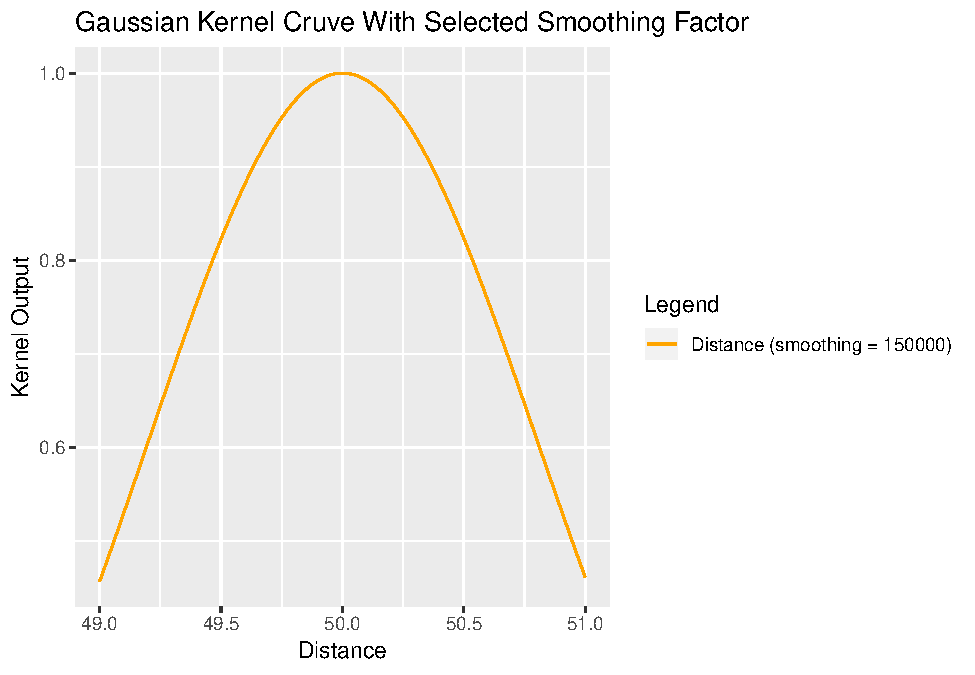
\includegraphics{lab03_files/figure-latex/unnamed-chunk-4-1.pdf}
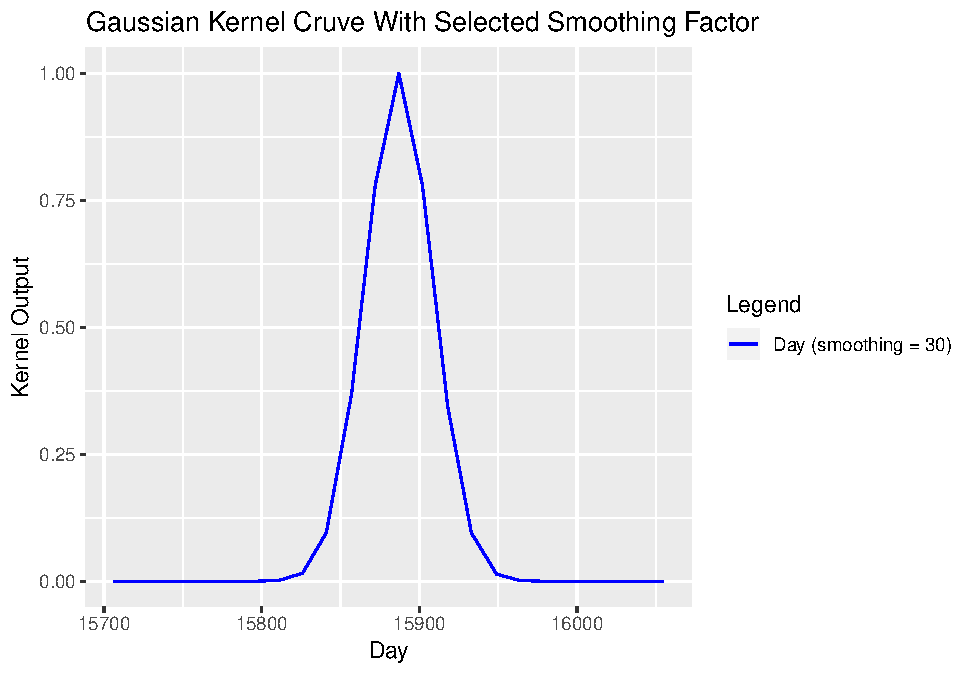
\includegraphics{lab03_files/figure-latex/unnamed-chunk-4-2.pdf}
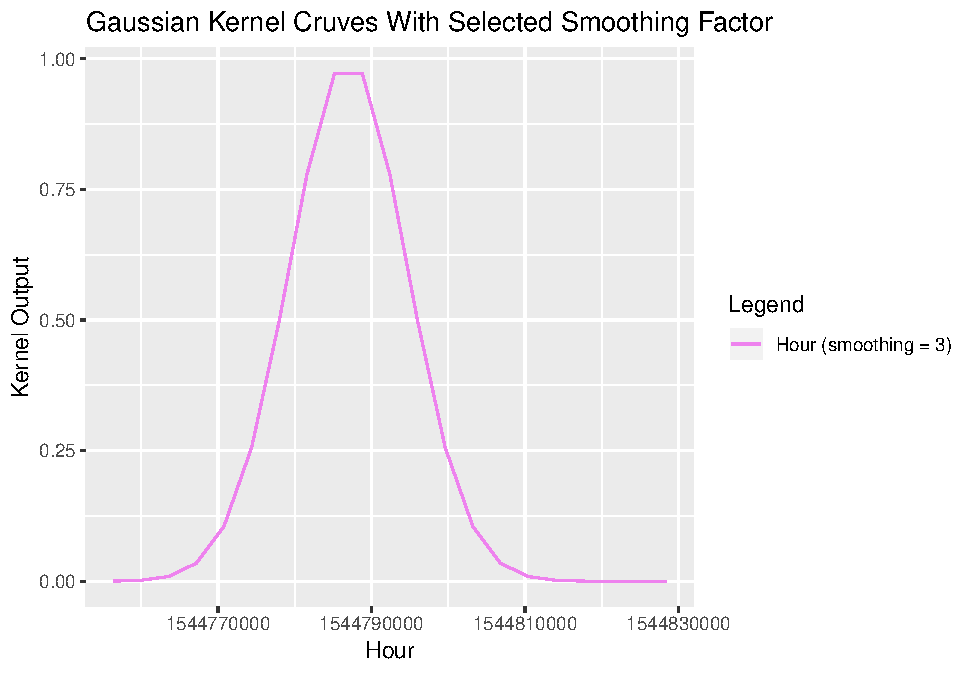
\includegraphics{lab03_files/figure-latex/unnamed-chunk-4-3.pdf}

\subsection{Weather Prediction}\label{weather-prediction}

For the weather prediction we use Linkoeping
(\texttt{latitude\ =\ 58.410809} and \texttt{longitude\ =\ 15.621373})
and as a date we use \texttt{date\ =\ "2000-05-08"} which is basically
random.

\textbf{Comment:} If we select an area or time where we basically have
no datapoints, all kernel functions return only \texttt{0}, so their sum
is zero as well. Dividing by zero is undefined and thus results in NA's.
\textbf{End Comment}

The following plot shows the weather prediction, we include the
predictions for the sum and the product of the three kernels. We observe
that the weather prediction seems to work better with the product of the
three kernels as the sum struggles in adjusting to the daily differences
in temperature. We can as well see that in general the prediction is
reasonable (it's colder at nights) and the temperature seems reasonable
as well (maybe not that much for the sum, but that's okay as it's not a
good model). The only ``akward'' thing to obersve is the ``bumby''
temperate drop at the end of the day.

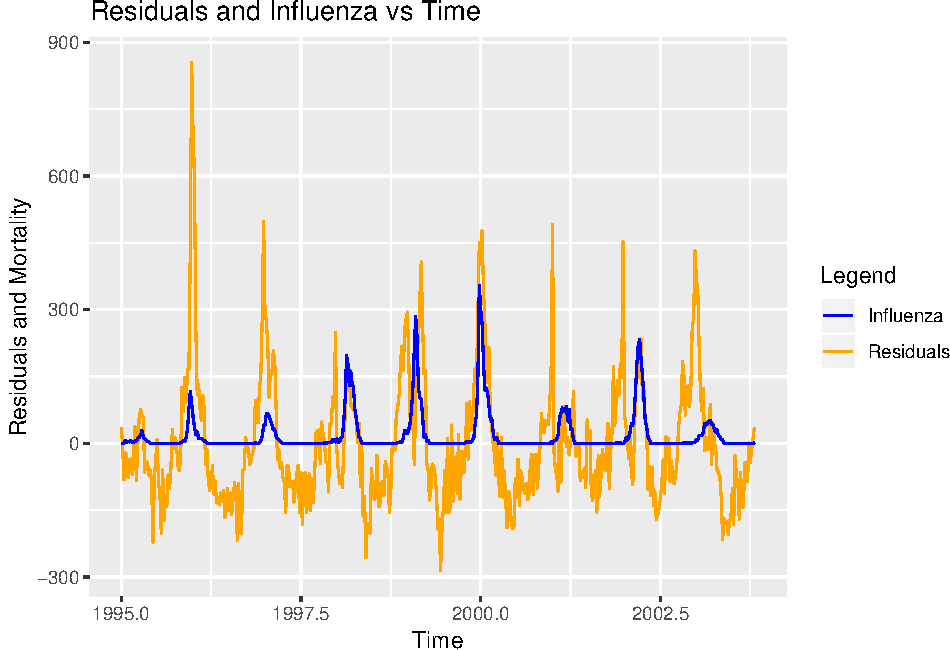
\includegraphics{lab03_files/figure-latex/unnamed-chunk-6-1.pdf}

\section{Support Vector Machines}\label{support-vector-machines}

\textbf{Task:}

Use the function ksvm from the R package kernlab to learn a SVM for
classifying the spam dataset that is included with the package. Consider
the radial basis function kernel (also known as Gaussian) with a width
of 0.05. For the C parameter, consider values 0.5, 1 and 5. This implies
that you have to consider three models.

\begin{itemize}
\tightlist
\item
  Perform model selection, i.e.~select the most promising of the three
  models (use any method of your choice except cross-validation or
  nested cross-validation).
\item
  Estimate the generalization error of the SVM selected above (use any
  method of your choice except cross-validation or nested
  cross-validation).
\item
  Produce the SVM that will be returned to the user, i.e.~show the code.
\item
  What is the purpose of the parameter C?
\end{itemize}

\subsection{Model Selection by Generalization
Error}\label{model-selection-by-generalization-error}

The confusion matrices look like this (C = 0.5, C = 1, C = 5):

\begin{verbatim}
##          model_svm_05_prediction
##           nonspam spam
##   nonspam     819   27
##   spam        104  430
\end{verbatim}

\begin{verbatim}
##          model_svm_1_prediction
##           nonspam spam
##   nonspam     816   30
##   spam         88  446
\end{verbatim}

\begin{verbatim}
##          model_svm_5_prediction
##           nonspam spam
##   nonspam     814   32
##   spam         79  455
\end{verbatim}

The error rates are (\texttt{C\ =\ 0.5}, \texttt{C\ =\ 1},
\texttt{C\ =\ 5}):

\begin{verbatim}
## [1] 0.09492754
\end{verbatim}

\begin{verbatim}
## [1] 0.08550725
\end{verbatim}

\begin{verbatim}
## [1] 0.08043478
\end{verbatim}

Therefore we select the model where \texttt{C\ =\ 5}. It doesn't really
make sense to select a model just based on the training data, thats why
the two steps were combined and the generalization error was considered
using the test data set. We use the test data set to actually get a good
esimation of our model (holdout).

\subsection{Produce the SVM}\label{produce-the-svm}

\begin{verbatim}
## Support Vector Machine object of class "ksvm" 
## 
## SV type: C-svc  (classification) 
##  parameter : cost C = 5 
## 
## Gaussian Radial Basis kernel function. 
##  Hyperparameter : sigma =  0.05 
## 
## Number of Support Vectors : 831 
## 
## Objective Function Value : -891.6116 
## Training error : 0.018478
\end{verbatim}

\begin{verbatim}
## [1] "Error rate: 0.0839971035481535"
\end{verbatim}

\subsection{C Parameter}\label{c-parameter}

C defines the cost of the constraint violation penalty. The default
value is set to 1 and it is an factor added to the error function. This
means, for \texttt{C\ =\ 0.5} the errors are halved and for
\texttt{C\ =\ 5} they are five times as large. Keep in mind that we also
have \(\epsilon\) which defines the threshold, when an error is applied.
C must always be greater than 0, otherwise there would never be an
error. Normally C and \(\epsilon\) are selected by Cross-Validation.

\section{Appendix: Source Code}\label{appendix-source-code}

\begin{Shaded}
\begin{Highlighting}[]
\NormalTok{knitr}\OperatorTok{::}\NormalTok{opts_chunk}\OperatorTok{$}\KeywordTok{set}\NormalTok{(}\DataTypeTok{echo =} \OtherTok{FALSE}\NormalTok{, }\DataTypeTok{cache =} \OtherTok{TRUE}\NormalTok{)}
\KeywordTok{library}\NormalTok{(geosphere)}
\KeywordTok{library}\NormalTok{(ggplot2)}
\KeywordTok{library}\NormalTok{(kernlab)}


\NormalTok{################################################################################}
\CommentTok{# Kernel Methods}
\NormalTok{################################################################################}

\NormalTok{## Helper Functions}

\NormalTok{min_distance =}\StringTok{ }\ControlFlowTok{function}\NormalTok{(a, b, ringSize) \{}
  
\NormalTok{  boundOne =}\StringTok{ }\KeywordTok{sapply}\NormalTok{(b, }\DataTypeTok{FUN =} \ControlFlowTok{function}\NormalTok{(x) }\KeywordTok{abs}\NormalTok{(a }\OperatorTok{-}\StringTok{ }\NormalTok{x))}
\NormalTok{  boundTwo =}\StringTok{ }\KeywordTok{sapply}\NormalTok{(b, }\DataTypeTok{FUN =} \ControlFlowTok{function}\NormalTok{(x) }\KeywordTok{abs}\NormalTok{(a }\OperatorTok{+}\StringTok{ }\NormalTok{ringSize }\OperatorTok{-}\StringTok{ }\NormalTok{x))}
    
  \KeywordTok{return}\NormalTok{(}\KeywordTok{pmin}\NormalTok{(boundOne, boundTwo))}
\NormalTok{\}}


\NormalTok{## Kernels}
\NormalTok{## The definition for the Guassian Kernel is taken from the slides, page 6.}

\NormalTok{kernel_gauss_distance =}\StringTok{ }\ControlFlowTok{function}\NormalTok{(pointA, pointB, smoothing) \{}
  
  \CommentTok{# Use distHaversine() as a help}
\NormalTok{  m =}\StringTok{ }\KeywordTok{cbind}\NormalTok{(pointB}\OperatorTok{$}\NormalTok{longitude, pointB}\OperatorTok{$}\NormalTok{latitude)}
\NormalTok{  u =}\StringTok{ }\KeywordTok{distHaversine}\NormalTok{(m, }\KeywordTok{c}\NormalTok{(pointA}\OperatorTok{$}\NormalTok{longitude, pointA}\OperatorTok{$}\NormalTok{latitude))}
\NormalTok{  u =}\StringTok{ }\NormalTok{u }\OperatorTok{/}\StringTok{ }\NormalTok{smoothing}
  \KeywordTok{return}\NormalTok{(}\KeywordTok{exp}\NormalTok{(}\OperatorTok{-}\NormalTok{(u}\OperatorTok{^}\DecValTok{2}\NormalTok{)))}
\NormalTok{\}}

\NormalTok{kernel_gauss_day =}\StringTok{ }\ControlFlowTok{function}\NormalTok{(dayA, dayB, smoothing) \{}
  
\NormalTok{  dayA_in_days =}\StringTok{ }\KeywordTok{as.numeric}\NormalTok{(}\KeywordTok{strftime}\NormalTok{(}\KeywordTok{as.Date}\NormalTok{(dayA}\OperatorTok{$}\NormalTok{date), }\StringTok{'%j'}\NormalTok{))}
\NormalTok{  dayB_in_days =}\StringTok{ }\KeywordTok{as.numeric}\NormalTok{(}\KeywordTok{strftime}\NormalTok{(}\KeywordTok{as.Date}\NormalTok{(dayB}\OperatorTok{$}\NormalTok{date), }\StringTok{'%j'}\NormalTok{))}
  
\NormalTok{  u =}\StringTok{ }\KeywordTok{min_distance}\NormalTok{(dayA_in_days, dayB_in_days, }\DecValTok{365}\NormalTok{)}
\NormalTok{  u =}\StringTok{ }\NormalTok{u }\OperatorTok{/}\StringTok{ }\NormalTok{smoothing}
  \KeywordTok{return}\NormalTok{(}\KeywordTok{exp}\NormalTok{(}\OperatorTok{-}\NormalTok{(u}\OperatorTok{^}\DecValTok{2}\NormalTok{)))}
\NormalTok{\}}

\NormalTok{kernel_gauss_hour =}\StringTok{ }\ControlFlowTok{function}\NormalTok{ (hourA, hourB, smoothing) \{}
  
\NormalTok{  hourA_in_h =}\StringTok{ }\KeywordTok{sapply}\NormalTok{(hourA}\OperatorTok{$}\NormalTok{time, }\DataTypeTok{FUN =} \ControlFlowTok{function}\NormalTok{(x)}
    \KeywordTok{as.numeric}\NormalTok{(}\KeywordTok{difftime}\NormalTok{(}\KeywordTok{strptime}\NormalTok{(x, }\DataTypeTok{format =} \StringTok{"%H:%M:%S"}\NormalTok{),}
                        \KeywordTok{strptime}\NormalTok{(}\StringTok{"00:00:00"}\NormalTok{, }\DataTypeTok{format =} \StringTok{"%H:%M:%S"}\NormalTok{))))}
  
\NormalTok{  hourB_in_h =}\StringTok{ }\KeywordTok{sapply}\NormalTok{(hourB}\OperatorTok{$}\NormalTok{time, }\DataTypeTok{FUN =} \ControlFlowTok{function}\NormalTok{(x)}
    \KeywordTok{as.numeric}\NormalTok{(}\KeywordTok{difftime}\NormalTok{(}\KeywordTok{strptime}\NormalTok{(x, }\DataTypeTok{format =} \StringTok{"%H:%M:%S"}\NormalTok{),}
                        \KeywordTok{strptime}\NormalTok{(}\StringTok{"00:00:00"}\NormalTok{, }\DataTypeTok{format =} \StringTok{"%H:%M:%S"}\NormalTok{))))}
  
\NormalTok{  u =}\StringTok{ }\KeywordTok{min_distance}\NormalTok{(hourA_in_h, hourB_in_h, }\DecValTok{24}\NormalTok{)}
\NormalTok{  u =}\StringTok{ }\NormalTok{u }\OperatorTok{/}\StringTok{ }\NormalTok{smoothing}
  \KeywordTok{return}\NormalTok{(}\KeywordTok{exp}\NormalTok{(}\OperatorTok{-}\NormalTok{(u}\OperatorTok{^}\DecValTok{2}\NormalTok{)))}
\NormalTok{\}}


\NormalTok{plot_values_distance =}\StringTok{ }\KeywordTok{list}\NormalTok{(}\DataTypeTok{latitude =} \KeywordTok{seq}\NormalTok{(}\DataTypeTok{from =} \DecValTok{49}\NormalTok{, }\DataTypeTok{to =} \DecValTok{51}\NormalTok{, }\DataTypeTok{by =} \FloatTok{0.01}\NormalTok{),}
                            \DataTypeTok{longitude =} \KeywordTok{seq}\NormalTok{(}\DataTypeTok{from =} \DecValTok{49}\NormalTok{, }\DataTypeTok{to =} \DecValTok{51}\NormalTok{, }\DataTypeTok{by =} \FloatTok{0.01}\NormalTok{))}

\NormalTok{plot_values_day =}
\StringTok{  }\KeywordTok{list}\NormalTok{(}\DataTypeTok{date =} \KeywordTok{c}\NormalTok{(}\StringTok{"2013-01-01"}\NormalTok{, }\StringTok{"2013-01-16"}\NormalTok{, }\StringTok{"2013-02-01"}\NormalTok{, }\StringTok{"2013-02-16"}\NormalTok{,}
                \StringTok{"2013-03-01"}\NormalTok{, }\StringTok{"2013-03-16"}\NormalTok{, }\StringTok{"2013-04-01"}\NormalTok{, }\StringTok{"2013-04-16"}\NormalTok{,}
                \StringTok{"2013-05-01"}\NormalTok{, }\StringTok{"2013-05-16"}\NormalTok{, }\StringTok{"2013-06-01"}\NormalTok{, }\StringTok{"2013-06-16"}\NormalTok{,}
                \StringTok{"2013-07-01"}\NormalTok{, }\StringTok{"2013-07-16"}\NormalTok{, }\StringTok{"2013-08-01"}\NormalTok{, }\StringTok{"2013-08-16"}\NormalTok{,}
                \StringTok{"2013-09-01"}\NormalTok{, }\StringTok{"2013-09-16"}\NormalTok{, }\StringTok{"2013-10-01"}\NormalTok{, }\StringTok{"2013-10-16"}\NormalTok{,}
                \StringTok{"2013-11-01"}\NormalTok{, }\StringTok{"2013-11-16"}\NormalTok{, }\StringTok{"2013-12-01"}\NormalTok{, }\StringTok{"2013-12-16"}\NormalTok{))}

\NormalTok{plot_values_hour =}
\StringTok{  }\KeywordTok{list}\NormalTok{(}\DataTypeTok{time =} \KeywordTok{c}\NormalTok{(}\StringTok{"04:00:00"}\NormalTok{, }\StringTok{"05:00:00"}\NormalTok{, }\StringTok{"06:00:00"}\NormalTok{, }\StringTok{"07:00:00"}\NormalTok{,}
                \StringTok{"08:00:00"}\NormalTok{, }\StringTok{"09:00:00"}\NormalTok{, }\StringTok{"10:00:00"}\NormalTok{, }\StringTok{"11:00:00"}\NormalTok{,}
                \StringTok{"12:00:00"}\NormalTok{, }\StringTok{"13:00:00"}\NormalTok{, }\StringTok{"14:00:00"}\NormalTok{, }\StringTok{"15:00:00"}\NormalTok{,}
                \StringTok{"16:00:00"}\NormalTok{, }\StringTok{"17:00:00"}\NormalTok{, }\StringTok{"18:00:00"}\NormalTok{, }\StringTok{"19:00:00"}\NormalTok{,}
                \StringTok{"20:00:00"}\NormalTok{, }\StringTok{"21:00:00"}\NormalTok{, }\StringTok{"22:00:00"}\NormalTok{, }\StringTok{"23:00:00"}\NormalTok{,}
                \StringTok{"24:00:00"}\NormalTok{))}

\NormalTok{compare_value_distance =}\StringTok{ }\KeywordTok{list}\NormalTok{(}\DataTypeTok{latitude =} \DecValTok{50}\NormalTok{, }\DataTypeTok{longitude =} \DecValTok{50}\NormalTok{)}
\NormalTok{compare_value_day =}\StringTok{ }\KeywordTok{list}\NormalTok{(}\DataTypeTok{date =} \StringTok{"2018-07-01"}\NormalTok{)}
\NormalTok{compare_value_hour =}\StringTok{ }\KeywordTok{list}\NormalTok{(}\DataTypeTok{time =} \StringTok{"12:30:00"}\NormalTok{)}

\CommentTok{# Smoothing factors}
\NormalTok{h_distance =}\StringTok{ }\DecValTok{150000} \CommentTok{#150000}
\NormalTok{h_date =}\StringTok{ }\DecValTok{30} \CommentTok{#30}
\NormalTok{h_time =}\StringTok{ }\DecValTok{3} \CommentTok{#3}

\NormalTok{distances =}\StringTok{ }\KeywordTok{kernel_gauss_distance}\NormalTok{(compare_value_distance,}
\NormalTok{                                 plot_values_distance, h_distance)}
\NormalTok{days =}\StringTok{ }\KeywordTok{kernel_gauss_day}\NormalTok{(compare_value_day, plot_values_day, h_date)}
\NormalTok{hours =}\StringTok{ }\KeywordTok{kernel_gauss_hour}\NormalTok{(compare_value_hour, plot_values_hour, h_time)}

\CommentTok{# Need to be continuous for plotting}
\NormalTok{plot_values_day =}\StringTok{ }\KeywordTok{as.numeric}\NormalTok{(}\KeywordTok{as.Date}\NormalTok{(plot_values_day}\OperatorTok{$}\NormalTok{date))}
\NormalTok{plot_values_hour =}
\StringTok{  }\KeywordTok{as.numeric}\NormalTok{(}\KeywordTok{strptime}\NormalTok{(plot_values_hour}\OperatorTok{$}\NormalTok{time, }\DataTypeTok{format =} \StringTok{"%H:%M:%S"}\NormalTok{))}

\CommentTok{# Dataframes for plotting}
\NormalTok{plot_data_frame_distance =}\StringTok{ }\KeywordTok{data.frame}\NormalTok{(plot_values_distance}\OperatorTok{$}\NormalTok{latitude, distances)}
\NormalTok{plot_data_frame_day =}\StringTok{ }\KeywordTok{data.frame}\NormalTok{(plot_values_day, days)}
\NormalTok{plot_data_frame_hour =}\StringTok{ }\KeywordTok{data.frame}\NormalTok{(plot_values_hour, hours)}


\KeywordTok{ggplot}\NormalTok{(plot_data_frame_distance) }\OperatorTok{+}
\StringTok{  }\KeywordTok{geom_line}\NormalTok{(}\KeywordTok{aes}\NormalTok{(}\DataTypeTok{x =}\NormalTok{ plot_values_distance}\OperatorTok{$}\NormalTok{latitude, }\DataTypeTok{y =}\NormalTok{ distances,}
                \DataTypeTok{colour =} \StringTok{"Distance (smoothing = 150000)"}\NormalTok{)) }\OperatorTok{+}
\StringTok{  }\KeywordTok{labs}\NormalTok{(}\DataTypeTok{title =} \StringTok{"Gaussian Kernel Distance"}\NormalTok{,}
       \DataTypeTok{y =} \StringTok{"Kernel Output"}\NormalTok{,}
       \DataTypeTok{x =} \StringTok{"Distance"}\NormalTok{, }\DataTypeTok{color =} \StringTok{"Legend"}\NormalTok{) }\OperatorTok{+}
\StringTok{  }\KeywordTok{scale_color_manual}\NormalTok{(}\DataTypeTok{values =} \KeywordTok{c}\NormalTok{(}\StringTok{"orange"}\NormalTok{))}
  
\KeywordTok{ggplot}\NormalTok{(plot_data_frame_day) }\OperatorTok{+}
\StringTok{  }\KeywordTok{geom_line}\NormalTok{(}\KeywordTok{aes}\NormalTok{(}\DataTypeTok{x =}\NormalTok{ plot_values_day,}
                \DataTypeTok{y =}\NormalTok{ days, }\DataTypeTok{colour =} \StringTok{"Day (smoothing = 30)"}\NormalTok{)) }\OperatorTok{+}
\StringTok{  }\KeywordTok{labs}\NormalTok{(}\DataTypeTok{title =} \StringTok{"Gaussian Kernel Over One Year"}\NormalTok{,}
       \DataTypeTok{y =} \StringTok{"Kernel Output"}\NormalTok{,}
       \DataTypeTok{x =} \StringTok{"Day"}\NormalTok{, }\DataTypeTok{color =} \StringTok{"Legend"}\NormalTok{) }\OperatorTok{+}
\StringTok{  }\KeywordTok{scale_color_manual}\NormalTok{(}\DataTypeTok{values =} \KeywordTok{c}\NormalTok{(}\StringTok{"blue"}\NormalTok{))}
  
\KeywordTok{ggplot}\NormalTok{(plot_data_frame_hour) }\OperatorTok{+}
\StringTok{  }\KeywordTok{geom_line}\NormalTok{(}\KeywordTok{aes}\NormalTok{(}\DataTypeTok{x =}\NormalTok{ plot_values_hour, }\DataTypeTok{y =}\NormalTok{ hours,}
                \DataTypeTok{colour =} \StringTok{"Hour (smoothing = 3)"}\NormalTok{)) }\OperatorTok{+}
\StringTok{  }\KeywordTok{labs}\NormalTok{(}\DataTypeTok{title =} \StringTok{"Gaussian Kernel Over One Day"}\NormalTok{,}
       \DataTypeTok{y =} \StringTok{"Kernel Output"}\NormalTok{,}
       \DataTypeTok{x =} \StringTok{"Hour"}\NormalTok{, }\DataTypeTok{color =} \StringTok{"Legend"}\NormalTok{) }\OperatorTok{+}
\StringTok{  }\KeywordTok{scale_color_manual}\NormalTok{(}\DataTypeTok{values =} \KeywordTok{c}\NormalTok{(}\StringTok{"violet"}\NormalTok{))}


\NormalTok{predict_weather =}\StringTok{ }\ControlFlowTok{function}\NormalTok{(u_latitude, u_longitude, u_date) \{}
  
  \CommentTok{# Data}
\NormalTok{  stations =}\StringTok{ }\KeywordTok{read.csv}\NormalTok{(}\StringTok{"stations.csv"}\NormalTok{, }\DataTypeTok{encoding =} \StringTok{"UTF-8"}\NormalTok{)}
\NormalTok{  temps =}\StringTok{ }\KeywordTok{read.csv}\NormalTok{(}\StringTok{"temps50k.csv"}\NormalTok{, }\DataTypeTok{encoding =} \StringTok{"UTF-8"}\NormalTok{)}
\NormalTok{  st =}\StringTok{ }\KeywordTok{merge}\NormalTok{(stations, temps, }\DataTypeTok{by=}\StringTok{"station_number"}\NormalTok{)}
  
  \CommentTok{# Filter all date posterior to the given date (doesn't make sense to predict}
  \CommentTok{# something that we already now)}
\NormalTok{  st =}\StringTok{ }\NormalTok{st[}\KeywordTok{as.Date}\NormalTok{(st}\OperatorTok{$}\NormalTok{date) }\OperatorTok{<}\StringTok{ }\KeywordTok{as.Date}\NormalTok{(u_date),]}
  
  \CommentTok{# Given Data}
  \CommentTok{# Each user input should be a list of:}
  \CommentTok{# latitude, longitude, date, time}
  \CommentTok{# time is created with the loop at we predict for every time for the given day}
  
  \CommentTok{# Times to predict}
  \CommentTok{#times = c("04:00:00", "05:00:00", "06:00:00", "07:00:00",}
  \CommentTok{#          "08:00:00", "09:00:00", "10:00:00", "11:00:00",}
  \CommentTok{#          "12:00:00", "13:00:00", "14:00:00", "15:00:00",}
  \CommentTok{#          "16:00:00", "17:00:00", "18:00:00", "19:00:00",}
  \CommentTok{#          "20:00:00", "21:00:00", "22:00:00", "23:00:00",}
  \CommentTok{#          "24:00:00")}
  
\NormalTok{  times =}\StringTok{ }\KeywordTok{c}\NormalTok{(}\StringTok{"04:00:00"}\NormalTok{, }\StringTok{"06:00:00"}\NormalTok{, }\StringTok{"08:00:00"}\NormalTok{,  }\StringTok{"10:00:00"}\NormalTok{, }
            \StringTok{"12:00:00"}\NormalTok{,  }\StringTok{"14:00:00"}\NormalTok{,}\StringTok{"16:00:00"}\NormalTok{,  }\StringTok{"18:00:00"}\NormalTok{,}
            \StringTok{"20:00:00"}\NormalTok{,  }\StringTok{"22:00:00"}\NormalTok{, }\StringTok{"24:00:00"}\NormalTok{)}
  
  \CommentTok{# Temperatures to predict}
\NormalTok{  temp =}\StringTok{ }\KeywordTok{data.frame}\NormalTok{()}
  
  \CommentTok{# Distance Kernel}
\NormalTok{  kernel_distance =}\StringTok{ }\KeywordTok{kernel_gauss_distance}\NormalTok{(}\KeywordTok{list}\NormalTok{(}
      \DataTypeTok{latitude =}\NormalTok{ u_latitude, }\DataTypeTok{longitude =}\NormalTok{ u_longitude), st, h_distance)}
  
  \CommentTok{# Day Kernel}
\NormalTok{  kernel_day =}\StringTok{ }\KeywordTok{kernel_gauss_day}\NormalTok{(}\KeywordTok{list}\NormalTok{(}\DataTypeTok{date =}\NormalTok{ u_date), st, h_date)}
  
  \CommentTok{# Prediction for each temp to predict}
  \ControlFlowTok{for}\NormalTok{ (i }\ControlFlowTok{in} \DecValTok{1}\OperatorTok{:}\KeywordTok{length}\NormalTok{(times)) \{}
    
    \CommentTok{# Hour Kernel}
\NormalTok{    kernel_hour =}\StringTok{ }\KeywordTok{kernel_gauss_hour}\NormalTok{(}\KeywordTok{list}\NormalTok{(}\DataTypeTok{time =}\NormalTok{ times[i]), st, h_time)}
    
\NormalTok{    kernel_sum =}\StringTok{ }\NormalTok{kernel_distance }\OperatorTok{+}\StringTok{ }\NormalTok{kernel_day }\OperatorTok{+}\StringTok{ }\NormalTok{kernel_hour}
\NormalTok{    kernel_prod =}\StringTok{ }\NormalTok{kernel_distance }\OperatorTok{*}\StringTok{ }\NormalTok{kernel_day }\OperatorTok{*}\StringTok{ }\NormalTok{kernel_hour}
    
    \CommentTok{# Now that we have the kernel value, we can calcuate the actual prediction}
    \CommentTok{# Formula taken from slide 8 from }
    \CommentTok{# "Histogram, Moving Window, and Kernel Regression"}
\NormalTok{    y_sum =}\StringTok{ }\NormalTok{kernel_sum }\OperatorTok\StringTok{ }\NormalTok{st}\OperatorTok{$}\NormalTok{air_temperature}\OperatorTok{/}\KeywordTok{sum}\NormalTok{(kernel_sum)}
\NormalTok{    y_prod =}\StringTok{ }\NormalTok{kernel_prod }\OperatorTok\StringTok{ }\NormalTok{st}\OperatorTok{$}\NormalTok{air_temperature}\OperatorTok{/}\KeywordTok{sum}\NormalTok{(kernel_prod)}
    
    \CommentTok{# Let's save this predicted temperature}
\NormalTok{    temp =}\StringTok{ }\KeywordTok{rbind}\NormalTok{(temp, }\KeywordTok{list}\NormalTok{(}\DataTypeTok{kernel_sum =}\NormalTok{ y_sum, }\DataTypeTok{kernel_prod =}\NormalTok{ y_prod))}
\NormalTok{  \}}
  \KeywordTok{return}\NormalTok{(}\KeywordTok{cbind}\NormalTok{(times, temp))}
\NormalTok{\}}

\KeywordTok{set.seed}\NormalTok{(}\DecValTok{1234567890}\NormalTok{)}

\CommentTok{# Linkoeping}
\NormalTok{latitude =}\StringTok{ }\FloatTok{58.4166}
\NormalTok{longitude =}\StringTok{ }\FloatTok{15.6333}
\NormalTok{date =}\StringTok{ "2000-05-08"}
\CommentTok{#date = "2018-12-14"}


\CommentTok{# Students' code here}
\NormalTok{pred_temp_sum =}\StringTok{ }\KeywordTok{predict_weather}\NormalTok{(latitude, longitude, date)}

\NormalTok{plot_data_frame =}
\StringTok{  }\KeywordTok{data.frame}\NormalTok{(}\KeywordTok{as.POSIXct}\NormalTok{(}\KeywordTok{paste}\NormalTok{(date ,pred_temp_sum}\OperatorTok{$}\NormalTok{times),}
                        \DataTypeTok{format =} \StringTok{"%Y-%m-%d %H:%M"}\NormalTok{), pred_temp_sum[}\DecValTok{2}\OperatorTok{:}\DecValTok{3}\NormalTok{])}
\KeywordTok{colnames}\NormalTok{(plot_data_frame) =}\StringTok{ }\KeywordTok{c}\NormalTok{(}\StringTok{"hour"}\NormalTok{, }\StringTok{"predWithSum"}\NormalTok{, }\StringTok{"predWithProd"}\NormalTok{)}

\KeywordTok{ggplot}\NormalTok{(plot_data_frame) }\OperatorTok{+}
\StringTok{  }\KeywordTok{geom_line}\NormalTok{(}\KeywordTok{aes}\NormalTok{(}\DataTypeTok{x =}\NormalTok{ hour, }\DataTypeTok{y =}\NormalTok{ predWithSum, }\DataTypeTok{group =} \DecValTok{1}\NormalTok{,}
                \DataTypeTok{colour =} \StringTok{"Kernel Regression (Sum)"}\NormalTok{)) }\OperatorTok{+}
\StringTok{  }\KeywordTok{geom_point}\NormalTok{(}\KeywordTok{aes}\NormalTok{(}\DataTypeTok{x =}\NormalTok{ hour, }\DataTypeTok{y =}\NormalTok{ predWithSum), }\DataTypeTok{colour =} \StringTok{"orange"}\NormalTok{) }\OperatorTok{+}
\StringTok{  }\KeywordTok{geom_line}\NormalTok{(}\KeywordTok{aes}\NormalTok{(}\DataTypeTok{x =}\NormalTok{ hour, }\DataTypeTok{y =}\NormalTok{ predWithProd, }\DataTypeTok{group =} \DecValTok{1}\NormalTok{,}
                \DataTypeTok{colour =} \StringTok{"Kernel Regression (Prod)"}\NormalTok{)) }\OperatorTok{+}
\StringTok{  }\KeywordTok{geom_point}\NormalTok{(}\KeywordTok{aes}\NormalTok{(}\DataTypeTok{x =}\NormalTok{ hour, }\DataTypeTok{y =}\NormalTok{ predWithProd), }\DataTypeTok{colour =} \StringTok{"blue"}\NormalTok{) }\OperatorTok{+}
\StringTok{  }\KeywordTok{labs}\NormalTok{(}\DataTypeTok{title =} \StringTok{"Temperature Prediction with Kernel Regression (Sum and Prod)"}\NormalTok{,}
       \DataTypeTok{y =} \StringTok{"Temperature"}\NormalTok{, }\DataTypeTok{x =} \StringTok{"Hour of the Day"}\NormalTok{, }\DataTypeTok{color =} \StringTok{"Legend"}\NormalTok{) }\OperatorTok{+}
\StringTok{  }\KeywordTok{scale_color_manual}\NormalTok{(}\DataTypeTok{values =} \KeywordTok{c}\NormalTok{(}\StringTok{"blue"}\NormalTok{, }\StringTok{"orange"}\NormalTok{))}


\NormalTok{################################################################################}
\CommentTok{# Support Vector Machines}
\NormalTok{################################################################################}

\KeywordTok{data}\NormalTok{(spam)}
\NormalTok{n =}\StringTok{ }\KeywordTok{dim}\NormalTok{(spam)[}\DecValTok{1}\NormalTok{]}
\KeywordTok{set.seed}\NormalTok{(}\DecValTok{12345}\NormalTok{)}
\NormalTok{id =}\StringTok{ }\KeywordTok{sample}\NormalTok{(}\DecValTok{1}\OperatorTok{:}\NormalTok{n, }\KeywordTok{floor}\NormalTok{(n}\OperatorTok{*}\FloatTok{0.4}\NormalTok{))}
\NormalTok{train_spam =}\StringTok{ }\NormalTok{spam[id,]}
\NormalTok{id1 =}\StringTok{ }\KeywordTok{setdiff}\NormalTok{(}\DecValTok{1}\OperatorTok{:}\NormalTok{n, id)}
\KeywordTok{set.seed}\NormalTok{(}\DecValTok{12345}\NormalTok{)}
\NormalTok{id2 =}\StringTok{ }\KeywordTok{sample}\NormalTok{(id1, }\KeywordTok{floor}\NormalTok{(n}\OperatorTok{*}\FloatTok{0.3}\NormalTok{))}
\NormalTok{val_spam =}\StringTok{ }\NormalTok{spam[id2,]}
\NormalTok{id3 =}\StringTok{ }\KeywordTok{setdiff}\NormalTok{(id1,id2)}
\NormalTok{test_spam =}\StringTok{ }\NormalTok{spam[id3,]}

\CommentTok{# Our three models depending on}
\NormalTok{model_svm_}\DecValTok{05}\NormalTok{ =}
\StringTok{  }\KeywordTok{ksvm}\NormalTok{(type }\OperatorTok{~}\StringTok{ }\NormalTok{., train_spam, }\DataTypeTok{kernel =} \StringTok{"rbfdot"}\NormalTok{,}
       \DataTypeTok{kpar =} \KeywordTok{list}\NormalTok{(}\DataTypeTok{sigma =} \FloatTok{0.05}\NormalTok{), }\DataTypeTok{C =} \FloatTok{0.5}\NormalTok{)}
\NormalTok{model_svm_}\DecValTok{1}\NormalTok{ =}
\StringTok{  }\KeywordTok{ksvm}\NormalTok{(type }\OperatorTok{~}\StringTok{ }\NormalTok{., train_spam, }\DataTypeTok{kernel =} \StringTok{"rbfdot"}\NormalTok{,}
       \DataTypeTok{kpar =} \KeywordTok{list}\NormalTok{(}\DataTypeTok{sigma =} \FloatTok{0.05}\NormalTok{), }\DataTypeTok{C =} \DecValTok{1}\NormalTok{)}
\NormalTok{model_svm_}\DecValTok{5}\NormalTok{ =}
\StringTok{  }\KeywordTok{ksvm}\NormalTok{(type }\OperatorTok{~}\StringTok{ }\NormalTok{., train_spam, }\DataTypeTok{kernel =} \StringTok{"rbfdot"}\NormalTok{,}
       \DataTypeTok{kpar =} \KeywordTok{list}\NormalTok{(}\DataTypeTok{sigma =} \FloatTok{0.05}\NormalTok{), }\DataTypeTok{C =} \DecValTok{5}\NormalTok{)}

\NormalTok{model_svm_05_prediction =}\StringTok{ }\KeywordTok{predict}\NormalTok{(model_svm_}\DecValTok{05}\NormalTok{, }\DataTypeTok{newdata =}\NormalTok{ val_spam)}
\NormalTok{model_svm_1_prediction =}\StringTok{ }\KeywordTok{predict}\NormalTok{(model_svm_}\DecValTok{1}\NormalTok{, }\DataTypeTok{newdata =}\NormalTok{ val_spam)}
\NormalTok{model_svm_5_prediction =}\StringTok{ }\KeywordTok{predict}\NormalTok{(model_svm_}\DecValTok{5}\NormalTok{, }\DataTypeTok{newdata =}\NormalTok{ val_spam)}

\NormalTok{cm_svm_}\DecValTok{05}\NormalTok{ =}\StringTok{ }\KeywordTok{table}\NormalTok{(val_spam}\OperatorTok{$}\NormalTok{type, model_svm_05_prediction)}
\NormalTok{cm_svm_}\DecValTok{1}\NormalTok{ =}\StringTok{ }\KeywordTok{table}\NormalTok{(val_spam}\OperatorTok{$}\NormalTok{type, model_svm_1_prediction)}
\NormalTok{cm_svm_}\DecValTok{5}\NormalTok{ =}\StringTok{ }\KeywordTok{table}\NormalTok{(val_spam}\OperatorTok{$}\NormalTok{type, model_svm_5_prediction)}

\NormalTok{error_svm_}\DecValTok{05}\NormalTok{ =}\StringTok{ }\DecValTok{1} \OperatorTok{-}\StringTok{ }\KeywordTok{sum}\NormalTok{(}\KeywordTok{diag}\NormalTok{(cm_svm_}\DecValTok{05}\NormalTok{)}\OperatorTok{/}\KeywordTok{sum}\NormalTok{(cm_svm_}\DecValTok{05}\NormalTok{))}
\NormalTok{error_svm_}\DecValTok{1}\NormalTok{ =}\StringTok{ }\DecValTok{1} \OperatorTok{-}\StringTok{ }\KeywordTok{sum}\NormalTok{(}\KeywordTok{diag}\NormalTok{(cm_svm_}\DecValTok{1}\NormalTok{)}\OperatorTok{/}\KeywordTok{sum}\NormalTok{(cm_svm_}\DecValTok{1}\NormalTok{))}
\NormalTok{error_svm_}\DecValTok{5}\NormalTok{ =}\StringTok{ }\DecValTok{1} \OperatorTok{-}\StringTok{ }\KeywordTok{sum}\NormalTok{(}\KeywordTok{diag}\NormalTok{(cm_svm_}\DecValTok{5}\NormalTok{)}\OperatorTok{/}\KeywordTok{sum}\NormalTok{(cm_svm_}\DecValTok{5}\NormalTok{))}


\KeywordTok{print}\NormalTok{(cm_svm_}\DecValTok{05}\NormalTok{)}
\KeywordTok{print}\NormalTok{(cm_svm_}\DecValTok{1}\NormalTok{)}
\KeywordTok{print}\NormalTok{(cm_svm_}\DecValTok{5}\NormalTok{)}


\KeywordTok{print}\NormalTok{(error_svm_}\DecValTok{05}\NormalTok{)}
\KeywordTok{print}\NormalTok{(error_svm_}\DecValTok{1}\NormalTok{)}
\KeywordTok{print}\NormalTok{(error_svm_}\DecValTok{5}\NormalTok{)}


\NormalTok{selected_model_prediction =}\StringTok{ }\KeywordTok{predict}\NormalTok{(model_svm_}\DecValTok{5}\NormalTok{, }\DataTypeTok{newdata =}\NormalTok{ test_spam)}

\NormalTok{cm_selected_model =}\StringTok{ }\KeywordTok{table}\NormalTok{(test_spam}\OperatorTok{$}\NormalTok{type, selected_model_prediction)}

\NormalTok{error_selected_model =}\StringTok{ }\DecValTok{1} \OperatorTok{-}\StringTok{ }\KeywordTok{sum}\NormalTok{(}\KeywordTok{diag}\NormalTok{(cm_selected_model)}\OperatorTok{/}\KeywordTok{sum}\NormalTok{(cm_selected_model))}

\KeywordTok{print}\NormalTok{(model_svm_}\DecValTok{5}\NormalTok{)}
\KeywordTok{print}\NormalTok{(}\KeywordTok{paste}\NormalTok{(}\StringTok{"Error rate:"}\NormalTok{, error_selected_model))}
\end{Highlighting}
\end{Shaded}


\end{document}
